% !TEX root = ../tex/6-3.tex
% 第6章：本文は青、補足は緑
\newcommand{\asmain}{%
    \setbeamercolor{frametitle}{fg=white,bg=main}%
    \setbeamercolor{structure}{fg=main}%
    \setbeamercolor{itemize item}{fg=main}%
    \setbeamercolor{itemize subitem}{fg=main}%
    \setbeamercolor{enumerate item}{fg=main}%
}
\newcommand{\assuppl}{%
    \setbeamercolor{frametitle}{fg=white,bg=examplecol}%
    \setbeamercolor{structure}{fg=examplecol}%
    \setbeamercolor{itemize item}{fg=examplecol}%
    \setbeamercolor{itemize subitem}{fg=examplecol}%
    \setbeamercolor{enumerate item}{fg=examplecol}%
}
% フレームタイトルの「補足」だけを□で囲む
\newcommand{\supplmark}{%
    \setlength{\fboxsep}{1.5pt}%
    \setlength{\fboxrule}{0.7pt}%
    \fbox{\textbf{補足}}%
}
\asmain


%=============================================
\begin{frame}{6.2から6.3へ}
    \begin{block}{ここまで（6.2）}
        訓練損失を式(6.2.5)のテンプレートに分解した。\\
        設計要素は (A) ノイズ日程、(B) 予測型、(C) 時間重み、(D) 時間分布。
    \end{block}
    \begin{block}{ここから（6.3）}
        (B) と (A) の\textbf{理論的同値}を精密化する。\\
        オラクルでは一致しても、学習モデルでは差が出うる、という線引き。
    \end{block}
\end{frame}
%=============================================
\asmain
\begin{frame}{6.3 の位置づけ}
    \begin{block}{この節の役割}
        予測型・PF-ODE・アフィン日程が「どこまで同じで、どこで違うか」を整理する
    \end{block}
    \begin{enumerate}
        \item \textbf{6.3.1} 四つの予測型の同値（命題6.3.1、図6.1）
        \item \textbf{6.3.2} パラメータ化ごとのPF-ODE（命題6.3.2）
        \item \textbf{6.3.3} すべてのアフィン流の同値（命題6.3.3、結論6.3.1--6.3.2）
        \item \textbf{6.3.4（補足）} 正準線形日程と$v$予測の利点
    \end{enumerate}
\end{frame}
%=============================================
\asmain
\begin{frame}{同値の四つの意味}
    論文はオラクル水準で、次を区別する。
    \begin{itemize}
        \item \textbf{予測}：$\bm{x}_t$と前向き日程があれば、\\
        clean / noise / score / velocity は代数的に相互変換できる
        \item \textbf{訓練目標}：二乗損失は正の時間依存因子だけ違い、\\
        点ごとのオラクル最小解は同じ
        \item \textbf{アフィン前向き過程}：$\bm{x}_t=\alpha_t\bm{x}_0+\sigma_t\veps$は、\\
        スケールと時間再パラメータで正準形へ写せる
        \item \textbf{周辺密度パス}：$\{p_t\}$が同じでも、\\
        決定／確率力学や軌跡は異なりうる
    \end{itemize}
\end{frame}
%=============================================
\asmain
\begin{frame}{理論の同値と実務の差}
    \begin{block}{オラクル}
        理想的な最小解どうしは情報同値。\\
        変換で同じPF-ODE速度を復元できる。
    \end{block}
    \begin{alertblock}{学習モデル}
        有限ネットは別関数を近似する。\\
        損失重み・最適化・離散化で訓練／標本化の挙動が変わる。
    \end{alertblock}
    \begin{exampleblock}{この節の進め方}
        予測 $\to$ PF-ODE $\to$ アフィン日程 $\to$（補足）正準形の利点
    \end{exampleblock}
\end{frame}
%=============================================
\section{6.3.1 四つの予測型}
\asmain
\begin{frame}{区切り：6.3.1 四つの予測型}
    \tableofcontents[currentsection]
\end{frame}
%=============================================
\asmain
\begin{frame}{コンポーネント(B)：予測型}
    式(6.2.5)の設計要素(B)を見る。\\
    よく使う四つのオラクル予測：
    \[
        \veps^\star(\vx_t,t),\quad
        \vx^\star(\vx_t,t),\quad
        s^\star(\vx_t,t),\quad
        v^\star(\vx_t,t).
    \]
    \begin{itemize}
        \item noise と clean は直接関係（§2.2.4）
        \item score と noise も直接関係（§3.4）
        \item いずれも同じ量の別の見方である
    \end{itemize}
\end{frame}
%=============================================
\asmain
\begin{frame}{命題6.3.1：パラメータ化の同値}
    \begin{block}{命題6.3.1（Equivalence of Parametrizations）}
        各目的関数を最小化するオラクルは、次で結ばれる：
        \[
            \veps^\star = -\sigma_t\, s^\star,
        \]
        \[
            \vx^\star
            =
            \frac{1}{\alpha_t}\vx_t
            +
            \frac{\sigma_t^{2}}{\alpha_t}\, s^\star,
            \tag{6.3.1}
        \]
        \[
            v^\star
            =
            \alpha_t'\vx^\star + \sigma_t'\veps^\star
            =
            f(t)\vx_t - \tfrac12 g^{2}(t)\, s^\star.
        \]
    \end{block}
\end{frame}
%=============================================
\asmain
\begin{frame}{命題6.3.1の読み方}
    $f(t),g(t)$は補題4.5.1経由で$\alpha_t,\sigma_t$と結ぶ。\\
    これらの最小解は式(6.2.1)--(6.2.4)の恒等式も満たす。
    \begin{exampleblock}{オラクル情報の同値}
        あるノイズ水準で一つのオラクルを知れば、\\
        $\vx_t$と前向き日程から他も決まる。\\
        例：score $\Rightarrow$ 事後平均clean $\Rightarrow$ PF-ODE速度。
    \end{exampleblock}
\end{frame}
%=============================================
\asmain
\begin{frame}{図6.1：四つのオラクルの相互変換}
    \centering
    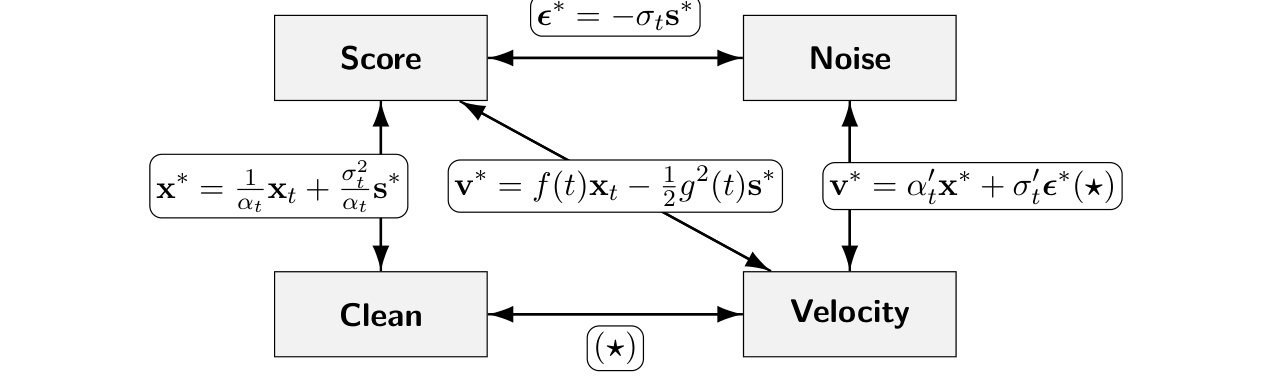
\includegraphics[width=0.92\textwidth,height=0.62\textheight,keepaspectratio]{fig-6-1.jpg}
\end{frame}
%=============================================
\asmain
\begin{frame}{図6.1の要点}
    \begin{itemize}
        \item Score $\leftrightarrow$ Noise：$\veps^\star=-\sigma_t s^\star$
        \item Score $\leftrightarrow$ Clean：Tweedie型の$\vx^\star$
        \item Velocity：$\alpha_t'\vx^\star+\sigma_t'\veps^\star$（$\star$）\\
        あるいは Score SDE 形 $f(t)\vx_t-\tfrac12 g^{2}(t)s^\star$
        \item clean と noise は $\vx_t=\alpha_t\vx^\star+\sigma_t\veps^\star$
    \end{itemize}
    \begin{block}{メッセージ}
        どの箱から出発しても、日程があれば他の箱へ移れる。
    \end{block}
\end{frame}
%=============================================
\asmain
\begin{frame}{ネット出力と変換}
    学習時に一次とする出力はどれでもよい：
    \[
        \veps_\phi,\quad
        \vx_\phi,\quad
        s_\phi,\quad
        v_\phi.
    \]
    一次出力を決めたら、式(6.3.1)と同じ代数で他を定義する。\\
    訓練済み$\phi_\times$では、変換後の予測は\textbf{構成上}ちょうど整合する：
    \[
        \vx
        =
        \alpha_t\,\vx_{\phi_\times}(\vx,t)
        +
        \sigma_t\,\veps_{\phi_\times}(\vx,t).
    \]
\end{frame}
%=============================================
\asmain
\begin{frame}{予測型と損失は別物}
    \begin{columns}[T,onlytextwidth]
        \begin{column}{0.48\textwidth}
            \begin{block}{ネットワーク出力}
                何を直接回帰するか\\
                （$\veps,x,s,v$）
            \end{block}
        \end{column}
        \begin{column}{0.48\textwidth}
            \begin{block}{損失に載せる量}
                出力を変換してから\\
                二乗誤差を測ってもよい
            \end{block}
        \end{column}
    \end{columns}
    \vfill
    変換は一般に時間依存の重みを変える（後の式(6.3.6)）。\\
    オラクルは情報同値でも、有限ネットでは表現・最適化が違う。
\end{frame}
%=============================================
\asmain
\begin{frame}{実務での使いどころ}
    \begin{itemize}
        \item noise予測 $\to$ reverse-SDE用のscoreへ変換
        \item 任意の予測 $\to$ PF-ODE用のvelocityへ変換
        \item 独立に訓練したモデルは、\\
        経験的予測や経験的PF-ODEが一致するとは限らない
    \end{itemize}
    \begin{alertblock}{命題の射程}
        同値は\textbf{理想オラクルの情報}について。\\
        出力パラメータ化と訓練目的は、なお独立な設計選択。
    \end{alertblock}
\end{frame}
%=============================================
\assuppl
\begin{frame}{\supplmark：証明の位置}
    証明は定理4.3.1（DSM下の大域最適）に近い。\\
    詳細は付録D.4。
    \begin{exampleblock}{ゼミでの扱い}
        スライドでは恒等式(6.3.1)と図6.1を本体とし、\\
        導出の細部は必要に応じて付録を参照する。
    \end{exampleblock}
\end{frame}
%=============================================
\asmain
\begin{frame}{6.3.1 のまとめ}
    \begin{itemize}
        \item 四つのオラクルは式(6.3.1)で相互変換できる（命題6.3.1）
        \item 図6.1がその関係の見取り図
        \item ネット出力と損失に載せる量は別設計
        \item 有限モデルでは「情報同値」が「実務同一」を意味しない
    \end{itemize}
    \begin{block}{次}
        同じオラクルを、PF-ODEの右辺として書き換える。
    \end{block}
\end{frame}
%=============================================
\section{6.3.2 PF-ODEの表現}
\asmain
\begin{frame}{区切り：6.3.2 PF-ODEの表現}
    \tableofcontents[currentsection]
\end{frame}
%=============================================
\asmain
\begin{frame}{なぜ表現を使い分けるか}
    PF-ODEはscore / noise / clean / velocityで書ける。\\
    原理上は交換可能でも、実務では次が変わる。
    \begin{itemize}
        \item ベクトル場の剛性（stiffness）
        \item 離散化誤差の出方
        \item 最適化のしやすさ
    \end{itemize}
    \begin{exampleblock}{典型的な選び方}
        高速ODE標本化（第9章）：$\veps$や$\vx$が多い。\\
        少数評価の生成器（第11章）：$\vx$や$v$が滑らかで有利なことが多い。
    \end{exampleblock}
\end{frame}
%=============================================
\asmain
\begin{frame}{命題6.3.2：四つのPF-ODE}
    \begin{block}{命題6.3.2（抜粋）}
        $\alpha_t'=\frac{d\alpha_t}{dt}$、$\sigma_t'=\frac{d\sigma_t}{dt}$として、経験的PF-ODEは同値：
        \[
            \frac{d\vx}{dt}
            =
            \frac{\alpha_t'}{\alpha_t}\vx
            -
            \sigma_t\!\left(\frac{\alpha_t'}{\alpha_t\sigma_t}-\frac{\sigma_t'}{\sigma_t}\right)\veps^\star,
        \]
        \[
            =
            \frac{\sigma_t'}{\sigma_t}\vx
            +
            \alpha_t\!\left(\frac{\alpha_t'}{\alpha_t\sigma_t}-\frac{\sigma_t'}{\sigma_t}\right)\vx^\star.
        \]
    \end{block}
\end{frame}
%=============================================
\asmain
\begin{frame}{命題6.3.2（続き）}
    score形とvelocity形：
    \[
        \frac{d\vx}{dt}
        =
        \frac{\alpha_t'}{\alpha_t}\vx
        +
        \sigma_t^{2}\!\left(\frac{\alpha_t'}{\alpha_t\sigma_t}-\frac{\sigma_t'}{\sigma_t}\right)s^\star,
        \tag{6.3.2}
    \]
    \[
        \frac{d\vx}{dt}
        =
        \alpha_t'\vx^\star + \sigma_t'\veps^\star
        =
        v^\star(\vx,t).
    \]
    \begin{block}{要点}
        最後の行が最も素直：$v$予測はODE右辺そのもの。
    \end{block}
\end{frame}
%=============================================
\asmain
\begin{frame}{Score SDE記法との接続}
    補題4.5.1に合わせ、
    \[
        f(t)=\frac{\alpha_t'}{\alpha_t},\qquad
        g^{2}(t)
        =
        \frac{d}{dt}\sigma_t^{2}
        -
        2\frac{\alpha_t'}{\alpha_t}\sigma_t^{2}
    \]
    とおくと、馴染みの形になる：
    \[
        \frac{d\vx}{dt}
        =
        f(t)\vx - \tfrac12 g^{2}(t)\, s^\star(\vx,t).
    \]
    \begin{exampleblock}{意味}
        命題6.3.1の$v^\star=f\vx-\tfrac12 g^{2}s^\star$と整合。\\
        予測型を変えても、オラクルのODEは同じ。
    \end{exampleblock}
\end{frame}
%=============================================
\asmain
\begin{frame}{離散化への橋}
    標本化では、この連続ODEを時間離散化する。\\
    代表例がDDIM更新（§9.2）で、EulerとPF-ODEが自然につながる。
    \begin{itemize}
        \item どの予測でも、変換後は同じオラクル場を指す
        \item ただし学習誤差とステップ誤差の出方は表現依存
    \end{itemize}
    \begin{block}{次}
        日程$(\alpha_t,\sigma_t)$そのものの同値へ進む（コンポーネントA）。
    \end{block}
\end{frame}
%=============================================
\asmain
\begin{frame}{6.3.2 のまとめ}
    \begin{itemize}
        \item PF-ODEは四つの予測で書ける（命題6.3.2）
        \item Score SDE形は補題4.5.1で回収される
        \item $v$形が右辺そのもの；他は線形項＋予測項に分解される
        \item 実務の選び方は剛性・誤差・最適化で決める
    \end{itemize}
\end{frame}
%=============================================
\section{6.3.3 アフィン流の同値}
\asmain
\begin{frame}{区切り：6.3.3 アフィン流の同値}
    \tableofcontents[currentsection]
\end{frame}
%=============================================
\asmain
\begin{frame}{コンポーネント(A)：ノイズ日程}
    式(6.2.5)の設計要素(A)を見る。\\
    一般のアフィン補間：
    \[
        \vx_t = \alpha_t\vx_0 + \sigma_t\veps.
    \]
    FM / RFでよく使う正準線形形：
    \[
        \vx_t^{\mathrm{FM}}
        =
        (1-t)\vx_0 + t\veps
        =
        \vx_0 + t(\veps-\vx_0),
    \]
    その速度は定数ベクトル$\veps-\vx_0$。
    \begin{block}{主張の核}
        この単純さは本質ではない。\\
        任意のアフィン補間は、正準パスの再スケール＋時間再パラメータ。
    \end{block}
\end{frame}
%=============================================
\asmain
\begin{frame}{状態レベルの書き換え}
    $c(t):=\alpha_t+\sigma_t\neq 0$、$\tau(t):=\sigma_t/(\alpha_t+\sigma_t)$とおくと
    \[
        \vx_t
        =
        (\alpha_t+\sigma_t)
        \Bigl(
            \tfrac{\alpha_t}{\alpha_t+\sigma_t}\vx_0
            +
            \tfrac{\sigma_t}{\alpha_t+\sigma_t}\veps
        \Bigr)
        =
        c(t)\,\vx_{\tau(t)}^{\mathrm{FM}}.
    \]
    \begin{itemize}
        \item 点ごとに、正準パスのスカラー倍
        \item $\tau$が連続かつ狭義単調なら、真の時間再パラメータでもある
        \item 通常の前向き日程ではSNR減少により$\tau$が単調になりやすい
    \end{itemize}
\end{frame}
%=============================================
\asmain
\begin{frame}{速度の変換}
    $\vx_t=c(t)\vx_{\tau(t)}^{\mathrm{FM}}$を時間微分すると
    \[
        v(\vx_t,t)
        =
        c'(t)\,\vx_{\tau(t)}^{\mathrm{FM}}
        +
        c(t)\,\tau'(t)\,
        v^{\mathrm{FM}}\!\bigl(\vx_{\tau(t)}^{\mathrm{FM}},\tau(t)\bigr).
    \]
    正準パス上では$v^{\mathrm{FM}}=-\vx_0+\veps$。
    \begin{exampleblock}{解釈}
        一般アフィンの速度 $=$ スケール変化の寄与 $+$\\
        正準速度を$\tau$で押し込んだ寄与。
    \end{exampleblock}
\end{frame}
%=============================================
\asmain
\begin{frame}{命題6.3.3：アフィン流の同値}
    \begin{block}{命題6.3.3（Equivalence of Affine Flows）}
        $\vx_t^{\mathrm{FM}}=(1-t)\vx_0+t\veps$、$\vx_t=\alpha_t\vx_0+\sigma_t\veps$、\\
        $c=\alpha+\sigma\neq 0$、$\tau=\sigma/(\alpha+\sigma)$とすると
        \[
            \vx_t = c(t)\,\vx_{\tau(t)}^{\mathrm{FM}},
            \tag{6.3.3}
        \]
        \[
            v(\vx_t,t)
            =
            c'(t)\vx_{\tau}^{\mathrm{FM}}
            +
            c(t)\tau'(t)\,
            v^{\mathrm{FM}}(\vx_{\tau}^{\mathrm{FM}},\tau).
        \]
        $\tau$が狭義単調なら、時間再パラメータ＋スカラー再スケールと読める。
    \end{block}
\end{frame}
%=============================================
\asmain
\begin{frame}{三角（trigonometric）流との同値}
    別の標準アフィン流（式(6.3.4)）：
    \[
        \vx_u^{\mathrm{Trig}}
        :=
        \cos(u)\,\vx_0 + \sin(u)\,\veps.
        \tag{6.3.4}
    \]
    $R_t:=\sqrt{\alpha_t^{2}+\sigma_t^{2}}>0$、$\cos\tau_t=\alpha_t/R_t$、$\sin\tau_t=\sigma_t/R_t$なら
    \[
        \vx_t
        =
        R_t\,\vx_{\tau_t}^{\mathrm{Trig}}.
        \tag{6.3.5}
    \]
    \begin{itemize}
        \item $(\alpha_t,\sigma_t)$を半径$R_t$と角度$\tau_t$に分解
        \item $\tau_t$が単調なら、これも時間再パラメータ
    \end{itemize}
\end{frame}
%=============================================
\asmain
\begin{frame}{三角流の速度}
    $u$についての微分：
    \[
        v_u^{\mathrm{Trig}}
        =
        -\sin(u)\,\vx_0 + \cos(u)\,\veps.
    \]
    式(6.3.5)と同じ変数変換で、速度（他のパラメータ化も同様）の\\
    閉じた変換が得られる。
    \begin{block}{結論6.3.1へ}
        VE / VP（三角を含む）/ FM / RF など、\\
        アフィン補間は日程によらず相互変換できる。
    \end{block}
\end{frame}
%=============================================
\asmain
\begin{frame}{結論6.3.1}
    \begin{block}{結論6.3.1}
        日程$(\alpha_t,\sigma_t)$がVE・VP（三角を含む）・FM・RFの\\
        いずれでも、アフィン補間は適切な時間変数の変更と\\
        スカラー再スケールで相互に変換できる。
    \end{block}
    \begin{exampleblock}{注意}
        「状態・速度のオラクル関係が写る」という意味。\\
        学習ダイナミクスや数値誤差まで同一とは限らない。
    \end{exampleblock}
\end{frame}
%=============================================
\asmain
\begin{frame}{四つの訓練目標の関係}
    $\sigma_t>0$、$\alpha_t'\sigma_t-\alpha_t\sigma_t'\neq 0$のもとで
    \[
        \veps^\star=\mathbb{E}[\veps|\vx_t],\quad
        \vx_0^\star=\mathbb{E}[\vx_0|\vx_t],\quad
        v^\star=\mathbb{E}[\alpha_t'\vx_0+\sigma_t'\veps|\vx_t].
    \]
    命題6.3.1より
    \[
        s^\star
        =
        -\frac{1}{\sigma_t}\veps^\star
        =
        \frac{\alpha_t}{\sigma_t^{2}}\vx_0^\star
        -
        \frac{\vx_t}{\sigma_t^{2}},
        \qquad
        v^\star=\alpha_t'\vx_0^\star+\sigma_t'\veps^\star.
    \]
\end{frame}
%=============================================
\asmain
\begin{frame}{ヘッド変換と損失の重み}
    ヘッドを
    \[
        s_\phi
        \equiv
        -\frac{1}{\sigma_t}\veps_\phi
        \equiv
        \frac{\alpha_t}{\sigma_t^{2}}
        \Bigl(\vx_\phi-\frac{\vx_t}{\alpha_t}\Bigr)
    \]
    のように揃えると、標本ごとの二乗損失は時間重みだけで結ばれる：
    \[
        \|s_\phi-\nabla\log p_t\|_{2}^{2}
        =
        \frac{1}{\sigma_t^{2}}\|\veps_\phi-\veps^\star\|_{2}^{2}
        =
        \frac{\alpha_t^{2}}{\sigma_t^{4}}\|\vx_\phi-\vx_0^\star\|_{2}^{2}
        \tag{6.3.6}
    \]
    （$v$形は$\sigma_t(\alpha_t'\sigma_t-\alpha_t\sigma_t')$の因子が入る）。
\end{frame}
%=============================================
\asmain
\begin{frame}{速度損失と正準形}
    命題6.3.3の$\vx_t=c(t)\vx_{\tau}^{\mathrm{FM}}$を使うと、
    \[
        \|v_\phi-v^\star\|_{2}^{2}
        =
        \bigl(c(t)\tau'(t)\bigr)^{2}
        \Bigl\|
            v_\phi^{\mathrm{FM}}\!\Bigl(\tfrac{\vx_t}{c},\tau\Bigr)
            -
            (v^{\mathrm{FM}})^\star\!\Bigl(\tfrac{\vx_t}{c},\tau\Bigr)
        \Bigr\|_{2}^{2}.
    \]
    \begin{block}{結論6.3.2}
        score / noise / clean / velocity の訓練目標は、\\
        $(\alpha_t,\sigma_t)$が決める時間依存重み（と$v$のアフィン変換）を除き\\
        理論的に同値である。
    \end{block}
\end{frame}
%=============================================
\asmain
\begin{frame}{6.3.3 のまとめ}
    \begin{itemize}
        \item 任意のアフィン流は正準FM形へ写せる（命題6.3.3）
        \item 三角流への半径・角度分解も同様（式(6.3.4)--(6.3.5)）
        \item 結論6.3.1：日程の見た目の差は再パラメータで吸収
        \item 結論6.3.2：四つの損失は時間重みの差を除き同値
    \end{itemize}
    \begin{block}{次（補足）}
        ではなぜ$(1-t,t)$と$v$予測が「自然」と言われるのか。
    \end{block}
\end{frame}
%=============================================
\section{6.3.4 正準流の解析（補足）}
\assuppl
\begin{frame}{\supplmark：区切り：6.3.4}
    \tableofcontents[currentsection]
\end{frame}
%=============================================
\assuppl
\begin{frame}{\supplmark：6.3.4の問い}
    四つのパラメータ化もアフィン日程も数学的には同値。\\
    それでも、\textbf{$v$予測＋正準線形日程}に利点はあるか？
    \begin{enumerate}
        \item \textbf{回帰目標と日程}：条件付き速度のスケール、曲率項
        \item \textbf{ソルバ含意}：数値積分との相性（詳細は第9章）
    \end{enumerate}
    \begin{exampleblock}{速度の二種}
        条件付き：$v_t(\vx_t|z)=\alpha_t'\vx_0+\sigma_t'\veps$（教師）\\
        周辺オラクル：$v^\star(\vx,t)=\mathbb{E}[v_t(\cdot|z)\mid\vx_t=\vx]$（推論）
    \end{exampleblock}
\end{frame}
%=============================================
\assuppl
\begin{frame}{\supplmark：線形日程の条件付き速度}
    $\alpha_t=1-\zeta(t)$、$\sigma_t=\zeta(t)$と書くと
    \[
        v_t(\vx_t|z)=\zeta'(t)\,(\veps-\vx_0).
    \]
    正準選択$\zeta(t)=t$なら$\zeta'=1$で、目標は時間に依存しない。
    \begin{block}{単位スケールの回帰目標（式(6.3.7)）}
        \[
            \mathbb{E}\|v_t(\cdot|z)\|_{2}^{2}
            =
            \mathbb{E}\|\veps\|_{2}^{2}+\mathbb{E}\|\vx_0\|_{2}^{2}
            =
            D+\mathrm{Tr}\,\mathrm{Cov}[\vx_0]+\|\mathbb{E}\vx_0\|_{2}^{2}.
        \]
        期待目標大きさは$t$に対して定数。
    \end{block}
\end{frame}
%=============================================
\assuppl
\begin{frame}{\supplmark：勾配安定性}
    データをゼロ平均・単位共分散に標準化すると、\\
    $\alpha_t'\vx_0$と$\sigma_t'\veps$が全$t$で同程度に寄与する。
    \[
        \mathcal{L}_{\mathrm{velocity}}(\phi)
        =
        \mathbb{E}_{t,\vx_0,\veps}
        \|v_\phi(\vx_t,t)-v_t(\vx_t|z)\|_{2}^{2}.
    \]
    勾配は目標$\|v_t\|_{2}$のスケールに敏感：\\
    端点で潰れる／爆発すると、勾配も消えやすい／跳ねやすい。
    \begin{exampleblock}{正準$\zeta(t)=t$の利点}
        回帰信号そのものからの端点崩壊・爆発がない。
    \end{exampleblock}
\end{frame}
%=============================================
\assuppl
\begin{frame}{\supplmark：曲率項の消滅}
    オラクル速度の分解：
    \[
        v^\star=\alpha_t'\vx^\star+\sigma_t'\veps^\star.
    \]
    固定$\vx$で時間微分すると
    \[
        \partial_t v^\star
        =
        \underbrace{\alpha_t''\vx^\star+\sigma_t''\veps^\star}_{\text{日程の曲率}}
        +
        \alpha_t'\partial_t\vx^\star+\sigma_t'\partial_t\veps^\star.
    \]
    線形$\alpha_t=1-t$、$\sigma_t=t$なら$\alpha_t''=\sigma_t''=0$。\\
    $v^\star$の時間変化は主に事後$\partial_t\vx^\star,\partial_t\veps^\star$を映す。
\end{frame}
%=============================================
\assuppl
\begin{frame}{\supplmark：$v$予測との相性}
    線形日程では$\alpha_t'=-1$、$\sigma_t'=+1$が定数。\\
    ドリフトに余分な$t$依存の再スケールが入らない。
    \begin{alertblock}{対比}
        score / $x_0$ / $\veps$ 形では、線形日程でも\\
        $\sigma_t'/\sigma_t$や$\alpha_t'/\alpha_t$が端点付近で急変しうる。
    \end{alertblock}
    排他的ではないが、$(1-t,t)+v$は時間依存が透明で安定しやすい。
\end{frame}
%=============================================
\assuppl
\begin{frame}{\supplmark：条件付きエネルギーの最小化}
    条件付き運動エネルギー（アフィン族内）：
    \[
        K[\zeta]
        :=
        \int_0^{1}
        \mathbb{E}\|v_t(\cdot|z)\|_{2}^{2}\,dt
        \propto
        \int_0^{1}\bigl(\zeta'(t)\bigr)^{2}\,dt.
    \]
    境界$\zeta(0)=0$、$\zeta(1)=1$のもとでEuler--Lagrangeは$\zeta''=0$。\\
    よって最小解は$\zeta(t)=t$（直線条件付きパス）。
    \begin{exampleblock}{意味}
        アフィン族の中で、正準流は$x_0\to\veps$の最も省エネルギーな動き方。\\
        詳細は命題7.5.1へ。
    \end{exampleblock}
\end{frame}
%=============================================
\assuppl
\begin{frame}{\supplmark：周辺エネルギーの注意}
    $\zeta(t)=t$は常に条件付き速度エネルギーを最小化する。\\
    しかし周辺オラクル$v^\star$のエネルギー最小とは限らない。
    \[
        \bm{y}_u=(1-u)\vx_0+u\veps,\quad
        b_u(\bm{y})=\mathbb{E}[\veps-\vx_0\mid\bm{y}_u=\bm{y}],
    \]
    \[
        \kappa(u)=\mathbb{E}\|b_u(\bm{y}_u)\|_{2}^{2},\qquad
        v^\star(\vx,t)=\zeta'(t)\,b_{\zeta(t)}(\vx).
    \]
    周辺運動エネルギー
    $K_{\mathrm{marg}}[\zeta]=\int_0^{1}\kappa(\zeta(t))(\zeta'(t))^{2}\,dt$。
\end{frame}
%=============================================
\assuppl
\begin{frame}{\supplmark：周辺最小のスケジュール}
    $\kappa>0$と正則性のもとで最小条件は
    \[
        \kappa(\zeta(t))\bigl(\zeta'(t)\bigr)^{2}=\mathrm{const}
        \quad\Leftrightarrow\quad
        \zeta'(t)\propto\frac{1}{\sqrt{\kappa(\zeta(t))}}.
    \]
    \begin{itemize}
        \item $\kappa$が大きい所では遅く、小さい所では速く進む
        \item $\zeta(t)=t$が周辺最小になるのは$\kappa$が定数のときだけ
    \end{itemize}
    \begin{block}{対比}
        条件付き：線形が常に定数速の最小。\\
        周辺：パス上の$\kappa(u)$に依存する。
    \end{block}
\end{frame}
%=============================================
\assuppl
\begin{frame}{\supplmark：標本化で$v$が自然な理由}
    PF-ODE標本化は結局速度場を要する。\\
    $v$予測はネット出力がODE右辺そのもの。
    \[
        \frac{d\vx}{dt}=v_{\phi_\times}(\vx,t)\approx v^\star(\vx,t).
    \]
    $x$/$\veps$/$s$は、状態と予測の組み合わせで同じ$v^\star$を表す\\
    （式(6.3.2)；オラクルODE自体は不変）。
\end{frame}
%=============================================
\assuppl
\begin{frame}{\supplmark：線形項＋ネット項}
    $x$/$\veps$/$s$形は共通して
    \[
        \frac{d\vx}{dt}
        =
        \underbrace{L(t)\vx}_{\text{既知の線形項}}
        +
        \underbrace{N_{\phi_\times}(\vx,t)}_{\text{ネット依存項}}.
    \]
    例（$\veps$予測）：
    \[
        L=\frac{\alpha_t'}{\alpha_t},\quad
        N=-\sigma_t\Bigl(\frac{\alpha_t'}{\alpha_t\sigma_t}-\frac{\sigma_t'}{\sigma_t}\Bigr)\veps_{\phi_\times}.
    \]
    指数積分型ソルバ（DPM-Solverなど）がこの構造を利用する（第9章）。
\end{frame}
%=============================================
\assuppl
\begin{frame}{\supplmark：正準線形＋$v$とEuler}
    $\vx_t=(1-t)\vx_0+t\veps$なら、一つの$v$予測から端点が復元できる：
    \[
        \hat\vx_0=\vx_t-t\,v_{\phi_\times},\qquad
        \hat\veps=\vx_t+(1-t)v_{\phi_\times}.
    \]
    $t\to s$の一歩：
    \[
        (1-s)\hat\vx_0+s\hat\veps
        =
        \vx_t+(s-t)v_{\phi_\times},
    \]
    これは学習速度場の\textbf{素のEuler更新}そのもの。
\end{frame}
%=============================================
\assuppl
\begin{frame}{\supplmark：6.3.4の結論}
    $v$＋正準線形には、定数目標スケール・曲率ゼロ・ODEとの直結など\\
    理論的な利点がある。\\
    それでも万能ではない。
    \begin{itemize}
        \item アーキテクチャ、正規化、時間重み、サンプラ、guidance
        \item 正則化、データスケール、訓練予算
    \end{itemize}
    最適構成はデータと目的に依存し、検証とアブレーションで決める。
\end{frame}
%=============================================
\section{まとめ}
\asmain
\begin{frame}{区切り：6.3のまとめ}
    \tableofcontents[currentsection]
\end{frame}
%=============================================
\asmain
\begin{frame}{6.3 のまとめ（1）}
    \begin{itemize}
        \item \textbf{予測}：命題6.3.1と図6.1で四つのオラクルが同値
        \item \textbf{PF-ODE}：命題6.3.2で同じ場の四つの書き方
        \item \textbf{アフィン日程}：命題6.3.3で正準／三角形へ写せる
        \item \textbf{損失}：結論6.3.2で時間重みを除き同値
    \end{itemize}
\end{frame}
%=============================================
\asmain
\begin{frame}{6.3 のまとめ（2）}
    \begin{itemize}
        \item 同値はオラクル情報・周辺パス・人口目的の水準
        \item 有限ネット・重み・離散化では実務差が残る
        \item （補足）$(1-t,t)+v$は安定で透明だが、万能ではない
    \end{itemize}
    \begin{block}{次（6.4）}
        背後の共通言語として、Fokker--Planck／連続方程式を見る。
    \end{block}
\end{frame}
